%\documentclass[a4paper,twocolumn]{article} % Document type

\documentclass[a4paper,12pt,oneside,onecolumn]{article} % Document type

\usepackage[left=1.0in, right=1.0in, top=1.0in, bottom=1.0in]{geometry}

\ifx\pdfoutput\undefined
    %Use old Latex if PDFLatex does not work
   \usepackage[dvips]{graphicx}% To get graphics working
   \DeclareGraphicsExtensions{.eps} % Encapsulated PostScript
 \else
    %Use PDFLatex
   \usepackage[pdftex]{graphicx}% To get graphics working
   \DeclareGraphicsExtensions{.pdf,.jpg,.png,.mps} % Portable Document Format, Joint Photographic Experts Group, Portable Network Graphics, MetaPost
   \pdfcompresslevel=9
\fi

\usepackage{amsmath,amssymb}   % Contains mathematical symbols
\usepackage[ansinew]{inputenc} % Input encoding, identical to Windows 1252
\usepackage[english]{babel}    % Language
\usepackage[square,numbers]{natbib}     %Nice numbered citations
\bibliographystyle{plainnat}            %Sorted bibliography



\begin{document}               % Begins the document

\title{Homework 2 in EL2450 Hybrid and Embedded Control Systems}
\author{
  Ahmed Alhaidari \\ 901009-3335 \\ aalh@kth.se 
  \and 
  Yue Jiao \\ 911024-7799 \\ yj@kth.se
  }
%\date{2010-10-10}             % If you want to set the date yourself.

\maketitle                     % Generates the title

\section*{Task 1}
Rate Monotonic scheduling is the scheduling when all tasks always have the same fixed priorities. So the tasks with higher priorities always run before those with lower priorities.

\section*{Task 2}
Since the three tasks all have the execution time $C_i = 6 ms$ and they have sampling times $T_i = {20, 29, 35}ms$, the utilization factor $U$ can be calculated as following:
\begin{equation}
U = \sum_{i=1}^n \frac{C_i}{T_i} = \frac{6}{20} + \frac{6}{29} + \frac{6}{35} = 0.678 < 0.69
\end{equation}
Thus, the tasks are schedulable. The execution priorities for the tasks,$J_i$, are $J1>J2>J3$ since the sampling time, $T_i$, are $T1>T2>T3$. This means that $J_1$ is the first task to be executed then $J_2$ and lastly $J_1$ as shown in figure(\ref{fig:1})

\begin{figure}[H]
    \centering
    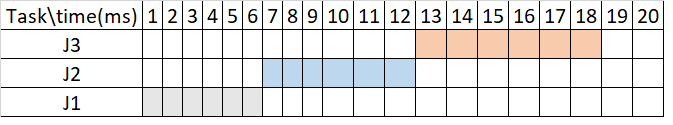
\includegraphics[scale=1]{Task_2.png}
    \caption{RM scheduling time line for 20ms}
    \label{fig:1}
\end{figure} 

\section*{Task 3}
The pendulums are stabilized. The results are shown in figure (\ref{fig:2}). The controller can easily stabilize the 3rd pendulum with the longest length than the other pendulums with the shorter lengths.

%the first controller is fastest and the last controller is slowest as expected. It is logical since the first controller always activates first.

\begin{figure}[H]
    \centering
    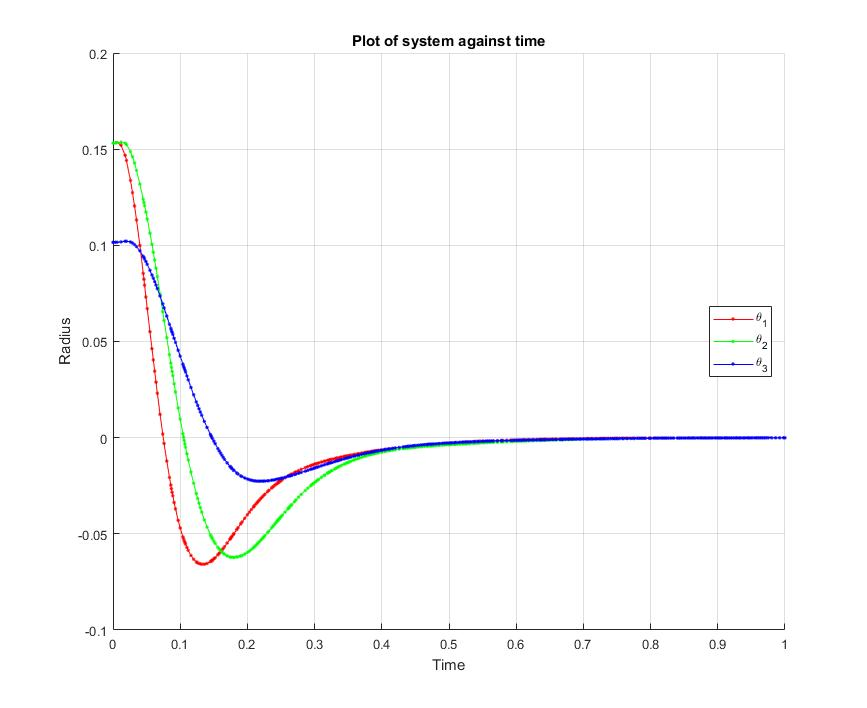
\includegraphics[scale=0.4]{theta06.jpg}
    \caption{Angles when the execution time is 6 ms}
    \label{fig:2}
\end{figure} 

\section*{Task 4}
The schedule is shown in figure (\ref{fig:3}). It can be seen that the tasks get time to execute before all their sampling times are over, see figure (\ref{fig:4}).

\begin{figure}[H]
    \centering
    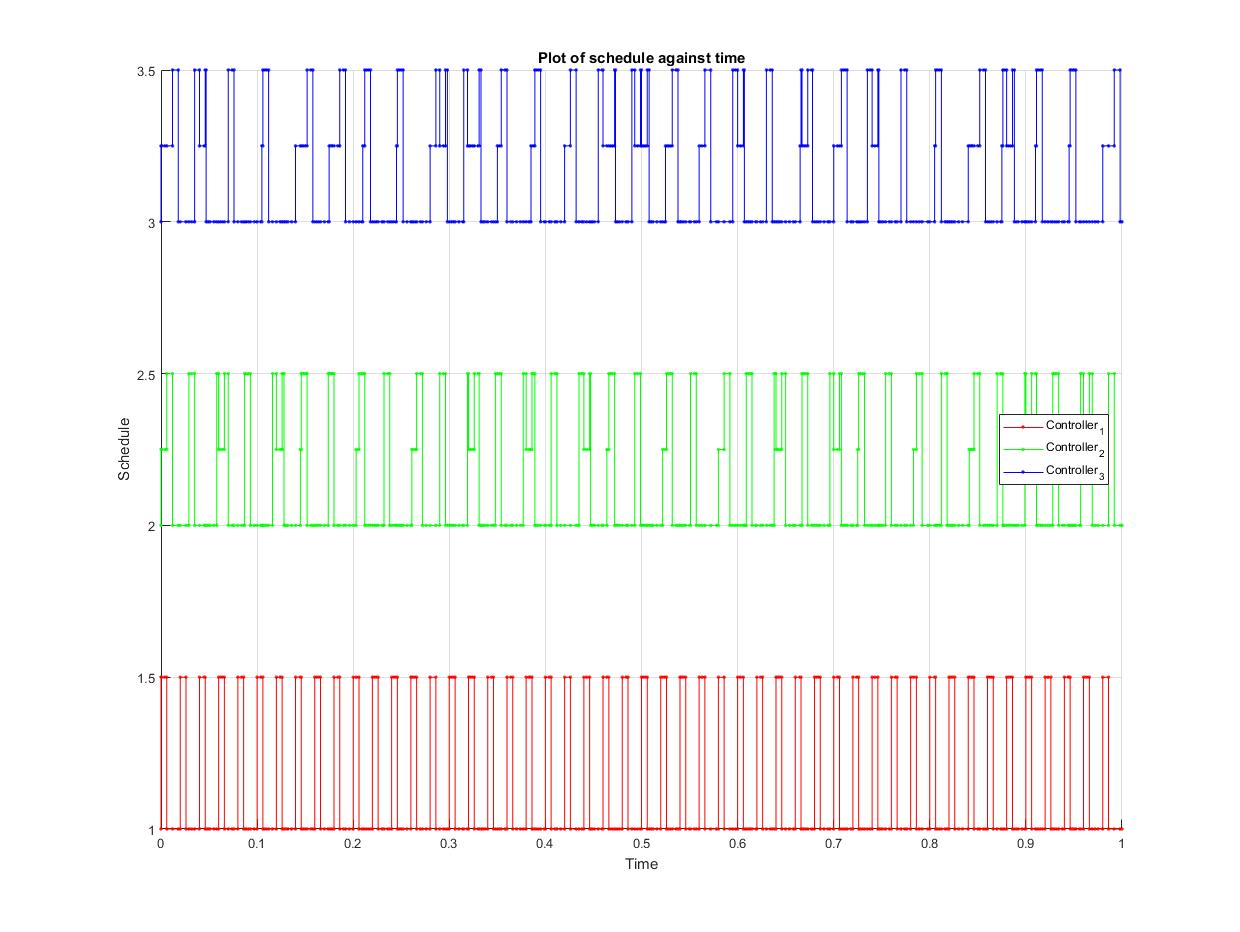
\includegraphics[scale=0.3]{schedule06.jpg}
    \caption{The rate monotonic scheduling with execution time 6 ms}
    \label{fig:3}
\end{figure}

\begin{figure}[H]
    \centering
    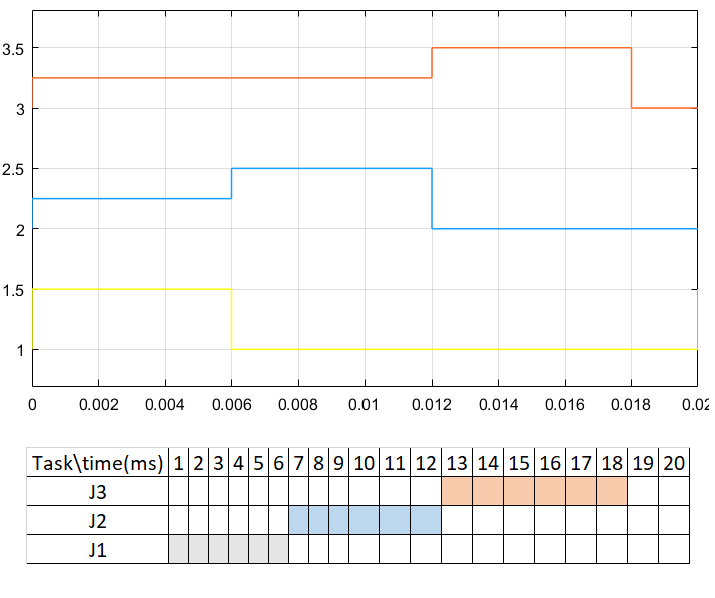
\includegraphics[scale=1]{Task_4.png}
    \caption{Comparing RM scheduling to the calculated one for $C=6ms$}
    \label{fig:4}
\end{figure}


\section*{Task 5}
Now instead, the execution time of the tasks become $C_i = 10 ms$. The utilization factor becomes: 
\begin{equation}
U = \sum_{i=1}^n \frac{C_i}{T_i} = \frac{10}{20} + \frac{10}{29} + \frac{10}{35} = 1.13 > 0.69
\end{equation}
So the the tasks are not schedulable in the sense of rate monotonic scheduling. 

As the plots in figure (\ref{fig:5}) show, it can be observed from the response of $\theta_3$ that third pendulum with the longest length is not stable. This happens because the 3rd pendulum does not have a time to be executed before the deadline is reached which is at 39ms, see figure(\ref{fig:6} $\&$ \ref{fig:7}). 


\begin{figure}[H]
    \centering
    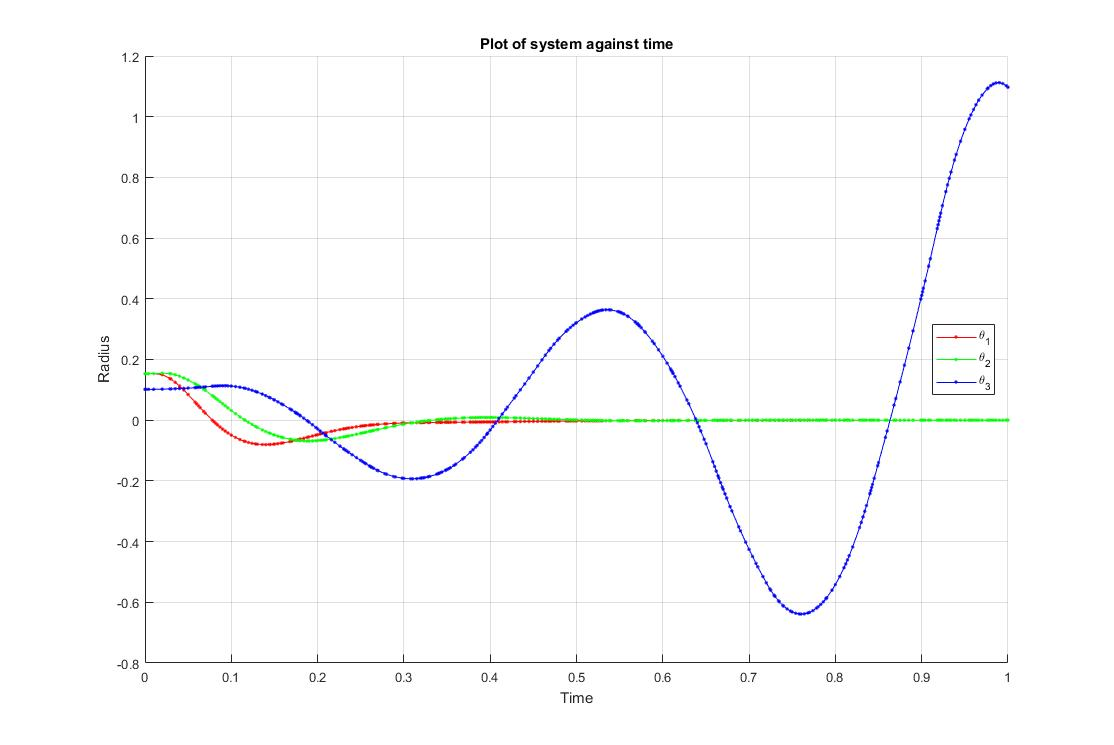
\includegraphics[scale=0.3]{theta10.jpg}
    \caption{Angles when the execution time is 10 ms}
    \label{fig:5}
\end{figure}

\begin{figure}[H]
    \centering
    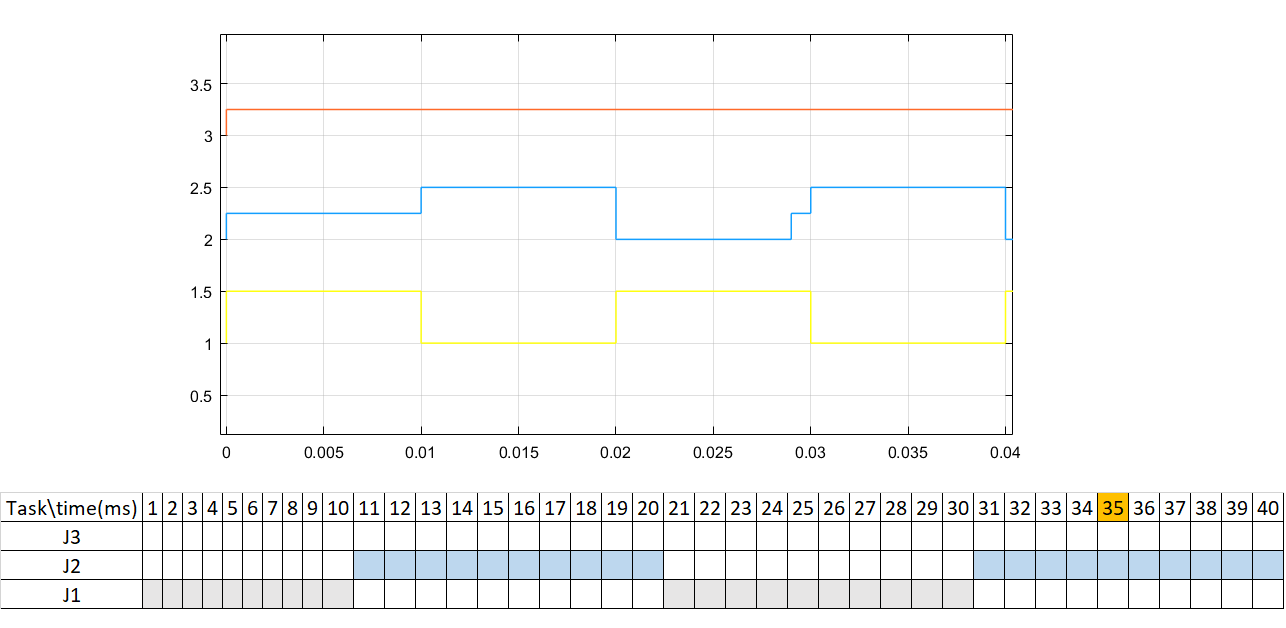
\includegraphics[scale=0.7]{Task_05.png}
    \caption{Comparing RM scheduling to the calculated one for $C=6ms$}
    \label{fig:6}
\end{figure}

\begin{figure}[H]
    \centering
    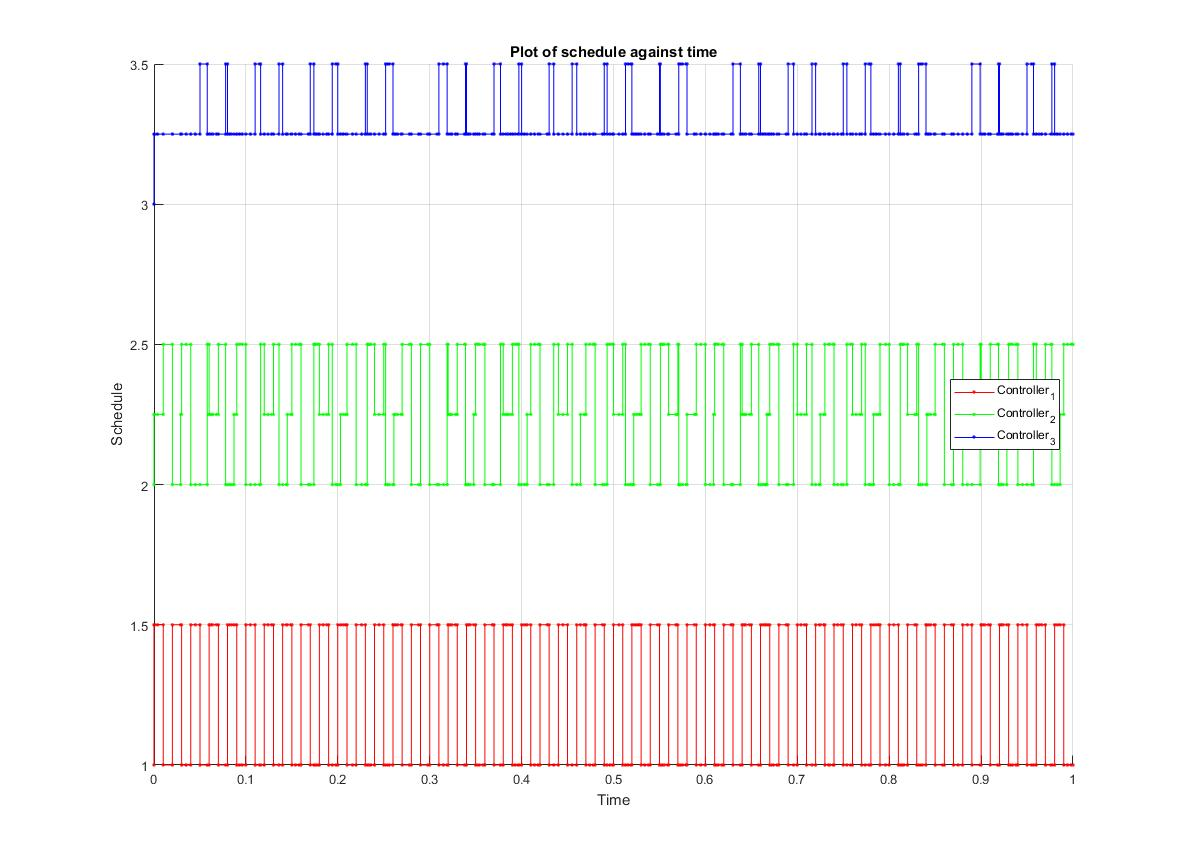
\includegraphics[scale=0.3]{schedule10.jpg}
    \caption{The rate monotonic scheduling with execution time 10 ms}
    \label{fig:7}
\end{figure}



\section*{Task 6}
The Earliest Deadline First scheduling is a scheduling that assign dynamic priorities to the tasks based on their absolute deadlines. This means that the one task with shortest time to deadline shall be executed. The advantage of usign EDF over the RM scheduling is that if the utilization factor $U\leq1$ then the one can conclude that the tasks are schedulable with EDF unlike the RM where it can be used even if the condition for $U$ is not met. Also, the EDF can works for aperiodic tasks. However, one of the disadvantages of using EDF scheduling is that it is more difficult to be implemented than rate monotonic scheduling since deadlines of all tasks need to be tracked through out the processing time.

%The advantage of this scheduling algorithm over rate monotonic scheduling is that it can be applied on large range of utilization factor, i.e. it is schedulable on all situation when $U \leq 1$ when rate monotonic scheduling works only when $U < 0.69$.


\section*{Task 7}
Since the utilization factor of the tasks when execution times are $6ms$ is $U = 0.678 < 1$, the tasks are schedulable in the sense of EDF scheduling. The first part of scheduling shall look like the following (see figure (\ref{fig:8})):

\begin{equation*}
\begin{aligned}
D_1 = 20, D_2 = 29, D_3 = 35  & \Rightarrow \textrm{Task 1 executed} \\ \Downarrow & \\ 
D_1 = 40, D_2 = 29, D_3 = 35  & \Rightarrow \textrm{Task 2 executed} \\ \Downarrow & \\ 
D_1 = 40, D_2 = 58, D_3 = 35  & \Rightarrow \textrm{Task 3 executed} \\ \Downarrow & \\ 
D_1 = 40, D_2 = 58, D_3 = 70  & \Rightarrow \textrm{Task 1 executed} \\ \Downarrow & \\ 
D_1 = 60, D_2 = 58, D_3 = 70  & \Rightarrow \textrm{Task 2 executed} \\ \Downarrow & \\ 
D_1 = 60, D_2 = 87, D_3 = 70  & \Rightarrow \textrm{Task 1 executed} \\ \Downarrow & \\ 
D_1 = 80, D_2 = 87, D_3 = 70  & \Rightarrow \textrm{Task 3 executed} \\ \Downarrow & \\ 
\vdots
\end{aligned}
\end{equation*}

\begin{figure}[H]
    \centering
    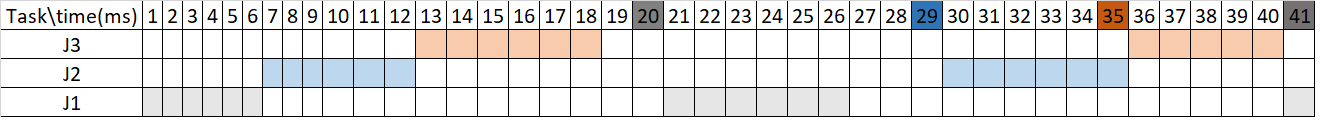
\includegraphics[scale=0.65]{Task_7.png}
    \caption{The EDF scheduling with execution time 6 ms}
    \label{fig:8}
\end{figure}

\section*{Task 8}
The pendulums are stable as shown in the plots of figure (\ref{fig:9}). The performance of the controller in this case where $C=6ms$ is similar to the RM scheduling case. The $1^{st}$ and the $2^{nd}$ pendulums need to go forth and back before they get stabilized while the $3^{rd}$ can easily be stabilized.
%Now it is easier to see that the first is clearly executed faster and the last task is executed slower. So the controller of pendulum 1 is more efficient in this case. 

\begin{figure}[H]
    \centering
    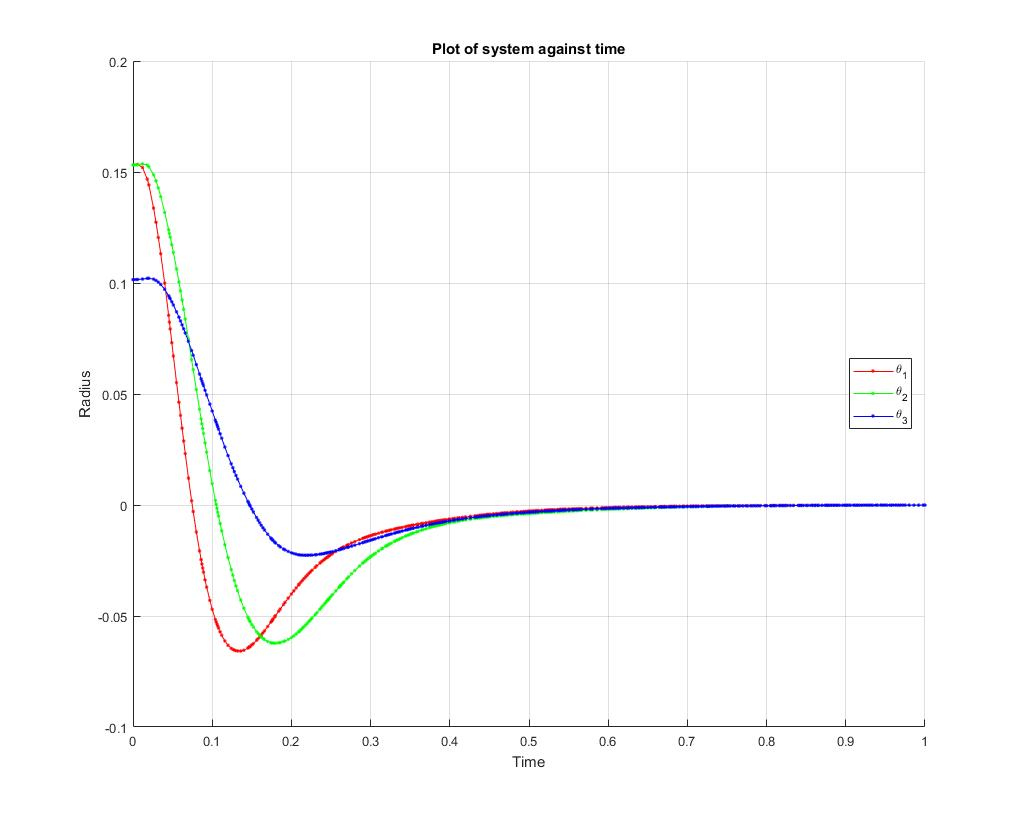
\includegraphics[scale=0.3]{theta06_EDF.jpg}
    \caption{Angles with EDF scheduling}
    \label{fig:9}
\end{figure}


\section*{Task 9}
It can be seen from the plots of the scheduling that the tasks do get time to execute before its sampling periods are over, see figures (\ref{fig:10} \& \ref{fig:11}). 

\begin{figure}[H]
    \centering
    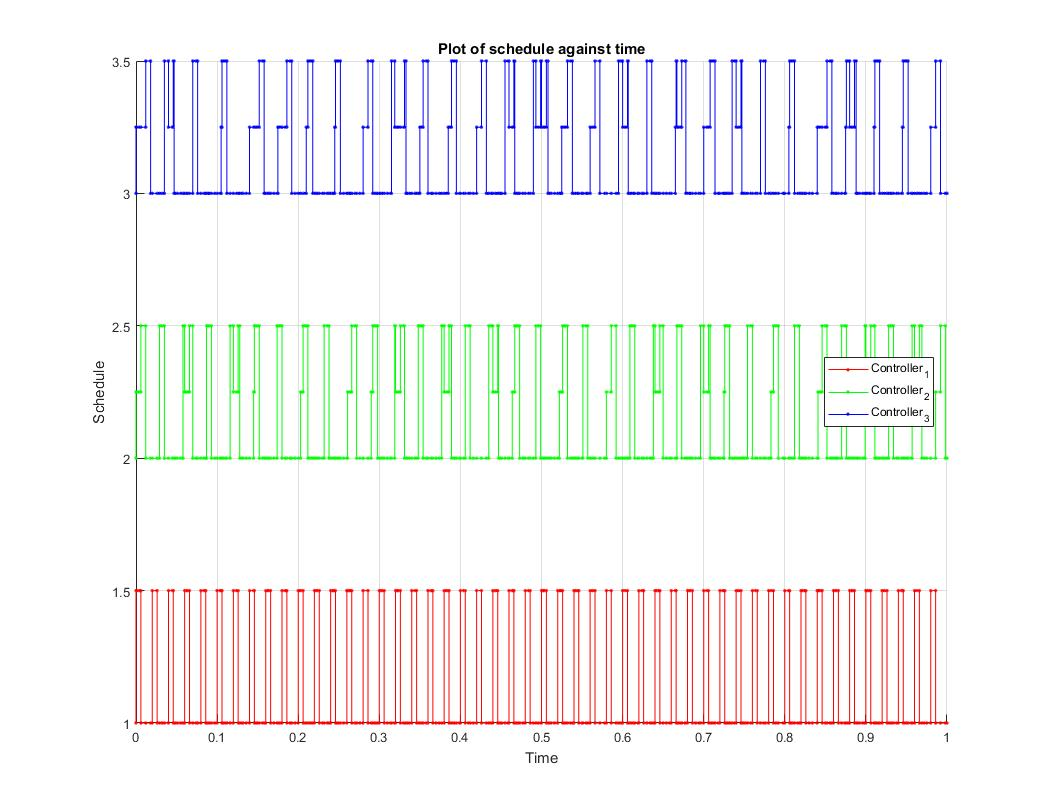
\includegraphics[scale=0.35]{schedule06_EDF.jpg}
    \caption{The EDF scheduling with execution time 6 ms}
    \label{fig:10}
\end{figure}

\begin{figure}[H]
    \centering
    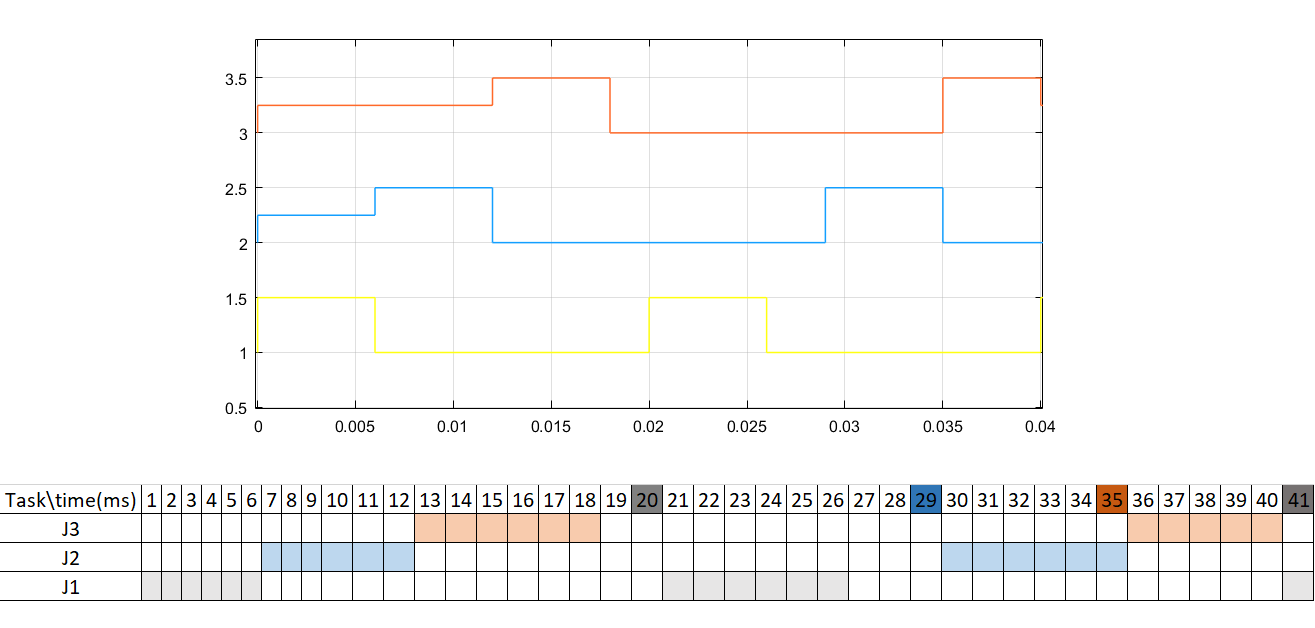
\includegraphics[scale=0.65]{Task_9.png}
    \caption{Comparing EDF scheduling to the calculated one for $C=6ms$}
    \label{fig:11}
\end{figure}


\section*{Task 10}
With execution time 10 ms and the EDF scheduling, the following results are shown in figures (\ref{fig:12},\ref{fig:13} \& \ref{fig:14}).

\begin{figure}[H]
    \centering
    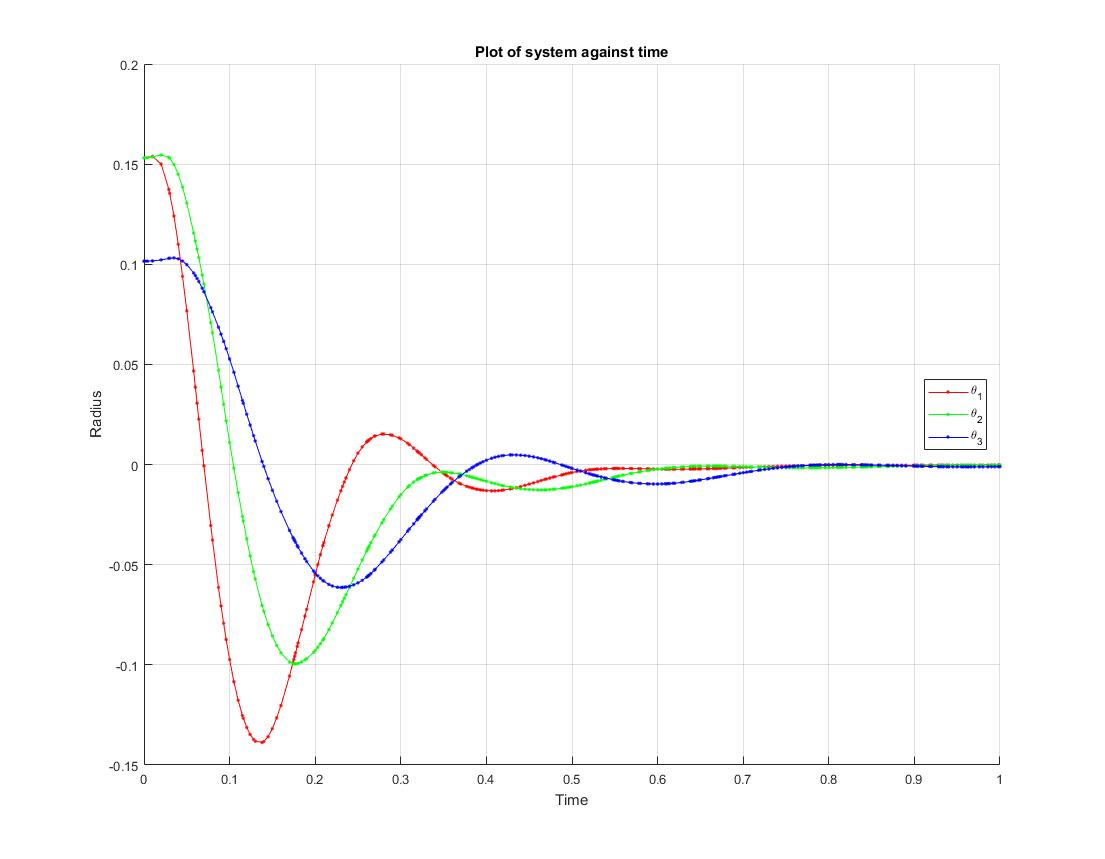
\includegraphics[scale=0.35]{theta10_EDF.jpg}
    \caption{Angles when the execution time is 10 ms}
    \label{fig:12}
\end{figure}

\begin{figure}[H]
    \centering
    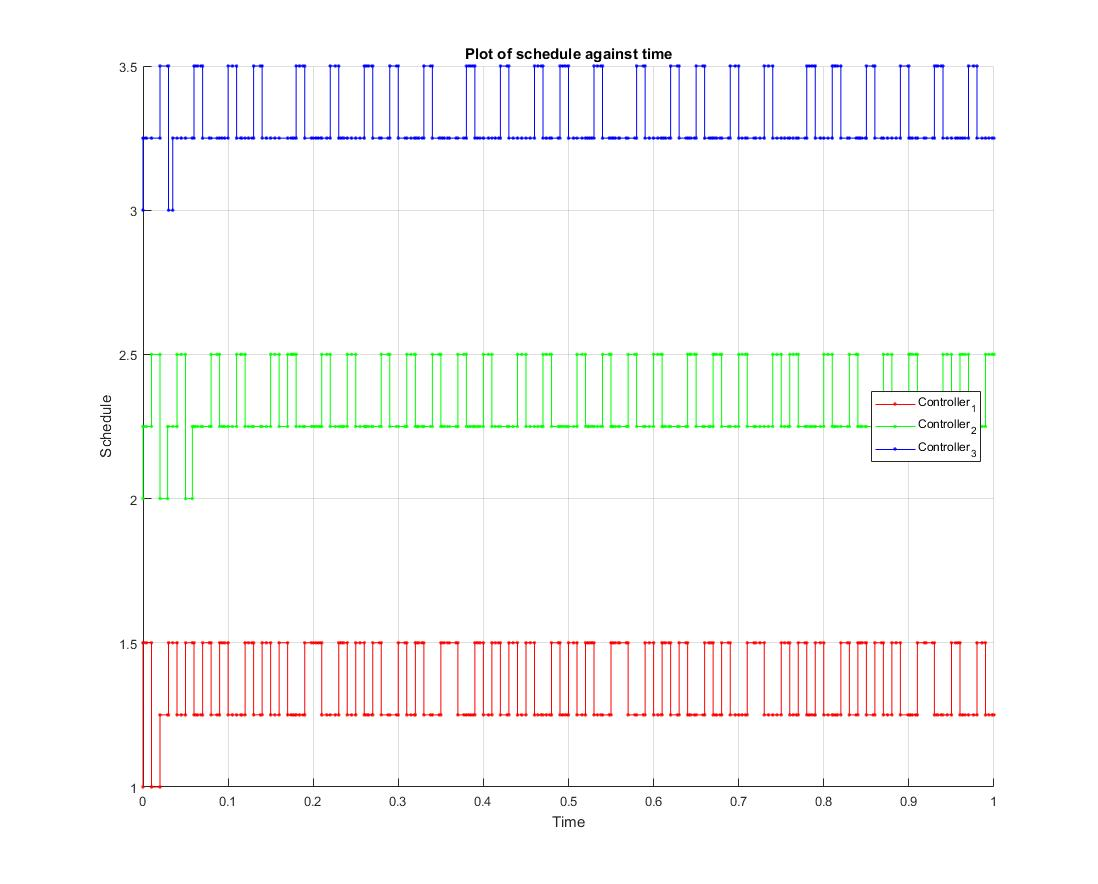
\includegraphics[scale=0.4]{schedule10_EDF.jpg}
    \caption{The EDF scheduling with execution time 10 ms}
    \label{fig:13}
\end{figure}

\begin{figure}[H]
    \centering
    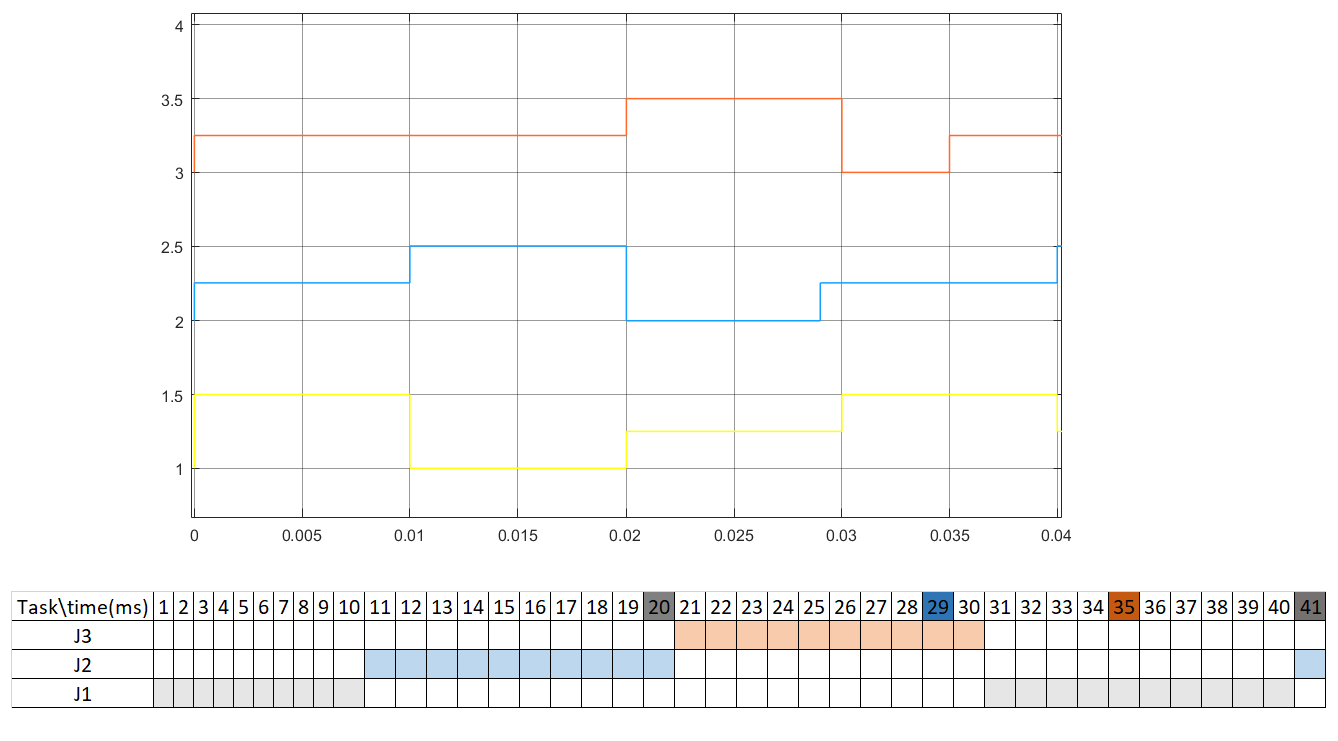
\includegraphics[scale=0.65]{Task_10.png}
    \caption{Comparing EDF scheduling to the calculated one for $C=10ms$}
    \label{fig:14}
\end{figure}


It can be seen that the system is still stable. However, the system take much longer time to get stabilized compared to the previous case with $C=6ms$ for the all of the three pendulums. As well, the $1^{st}$ pendulum almost oscillate between $0.15$ rad \& $-0.15$ rad before it get stabilized. Observing the scheduling behavior in this case,where the execution time is $10ms$, the one can notice that the CPU is never idle! Whenever the CPU finish computing one task, it starts with the second one immediately, see figure (\ref{fig:11} \& \ref{fig:14}). 

%it is slower than the system with execution time 6 ms of tasks and it is more oscillating. The scheduling looks like the scheduling with 6 ms execution time but now it is slower. 

\section*{Task 11}
First, let's consider the case where the computation time is $C=6ms$. The performance of the controllers for both scheduling algorithm are the same, and this can be seen in figure (\ref{fig:3} \& \ref{fig:8}) for RM and EDF respectively. Since the EDF scheduling requires a continuous observation, it is preferable to use RM which gives fixed priorities to the tasks. Now, considering the other case where the execution time is $C=10ms$. The controllers under the EDF scheduling is much better now since all the pendulums are stabilized, see figure(\ref{fig:5}). Unlike controller under the RM scheduling, only the $1^{st}$ \& $2^{nd}$ pendulums are stabilized while the $3^{rd}$ pendulum is not stable, see figure (\ref{fig:12}).

%The EDF scheduling does better than RM scheduling in a way that it is stable even when the execution time is larger. So the EDF scheduling is stable for more utilization factor than RM scheduling. But from the results, it can be observed that the EDF scheduling is slower than RM scheduling and it oscillates more as well. 

\section*{Task 12}

Since the delay $\tau=\tau_{sc} + \tau_{ca} \leq h$, the state space equations of the discrete time system can be written as follows: 
\begin{equation}
x(kh+h)= \phi x(kh) + \Gamma_0 u(kh) + \Gamma_1 u(kh-h)
\end{equation}
\begin{equation}
y(kh)=Cx(kh)
\end{equation}

For $A=0$ and $B=I$, 
\begin{align*}
\Phi = \mathrm{e}^{Ah}= I
\\\Gamma_0=\int\limits_{0}^{h-\tau} \mathrm{e}^{As} ds B = (h-\tau)I
\\\Gamma_1=\mathrm{e}^{A(h-\tau)}\int\limits_{0}^{\tau} \mathrm{e}^{As} ds B = \tau I
\end{align*}
So, the system equations are: 
\begin{equation}
x(kh+h)= x(kh) + (h-\tau) u(kh) + \tau u(kh-h)
\label{eq:06}
\end{equation}
\begin{equation} 
y(kh)=Cx(kh) 
\end{equation}

Now, the control law  $u(kh)=-Kx(kh)$ is substituted in equation (\ref{eq:06}), and the closed loop system equations are written in a matrix form as follows:

\[
\begin{bmatrix}
x(kh+h) \\ u(kh)
\end{bmatrix}
=
  \begin{bmatrix}
    1-hk+\tau K & \tau \\
    -K & 0
  \end{bmatrix}
  \begin{bmatrix}
    x(kh) \\
    u(kh-h)
  \end{bmatrix}
\]

% This part might be removed !!!
\begin{align*}
    y(kh)=-\frac{C}{K} u(kh)
\end{align*}

%%%%%%%%%%%%

\section*{Task 13}

The characteristic equation can be calculated as follows: 

\begin{align*}
    \phi`= \begin{bmatrix}
    1-hk+\tau K & \tau \\
    -K & 0
   \end{bmatrix}
\\ \\
det(z I -\phi`)=0
\\ \\
det(\begin{bmatrix}
    z & 0 \\
    0 & z
   \end{bmatrix} - \begin{bmatrix}
    1-hk+\tau K & \tau \\
    -K & 0
   \end{bmatrix}) =0
\\ \\
z^2 + z(hK-\tau K - 1)+\tau K =0
\end{align*} 

To find the condition that assure the stability of the system, , Routh-Hurwitz criterion for stability of the $2^{nd}$ order polynomials in discrete time ($a_2 z^2 + a_1 z + a_0$) is used as follows:
\begin{enumerate} 
\item $a_2-a_1+a_0 > 0$
\item $a_2-a_0 >0$
\item $a_2+a_1+a_0 > 0$
\end{enumerate} 

From the characteristic polynomials the coefficients are: 
\begin{align*}
a_2&=1 & a_1&=(hK -\tau K -1) & a_0&=\tau K
\end{align*} 

Now, substituting for the coefficients in 1,2,and 3 gives the following conditions: 
\begin{enumerate} 
\item $\frac{\tau}{h}>\frac{1}{2}-\frac{1}{hK}$
\item $\frac{\tau}{h}<\frac{1}{hK}$
\item $hK>0$

Since the delay $0 \leq \tau < h$, the condition of the stability of the system can be written in the following format: 

\begin{align*}
\frac{1}{2}-\frac{1}{hK} <\frac{\tau}{h} < \frac{1}{hK}
\end{align*}
or
\begin{align*}
max\{\frac{1}{2}-\frac{1}{hK},0\} <\frac{\tau}{h} < min\{1,\frac{1}{hK}\}
\end{align*} 

\end{enumerate} 

\section*{Task 14}

The system is unstable for $ \tau > 0.04$, see figures (\ref{fig:15}-\ref{fig:18}).

\begin{figure}[H]
    \centering
    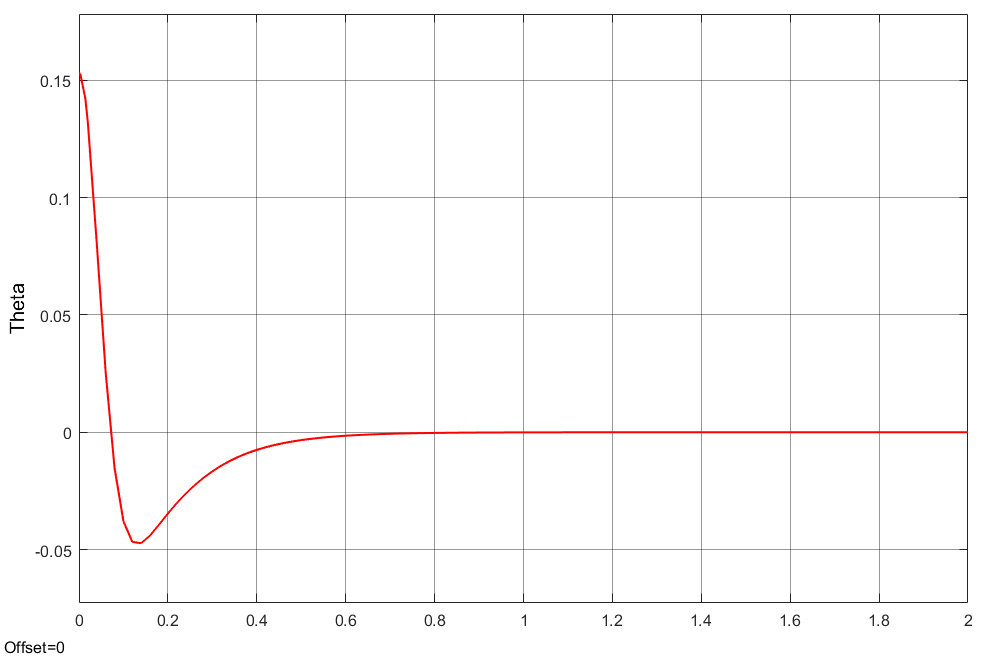
\includegraphics[scale=0.5]{Task_14_00.png}
    \caption{The step response of the system with $\tau=0$}
    \label{fig:15}
\end{figure}

\begin{figure}[H]
    \centering
    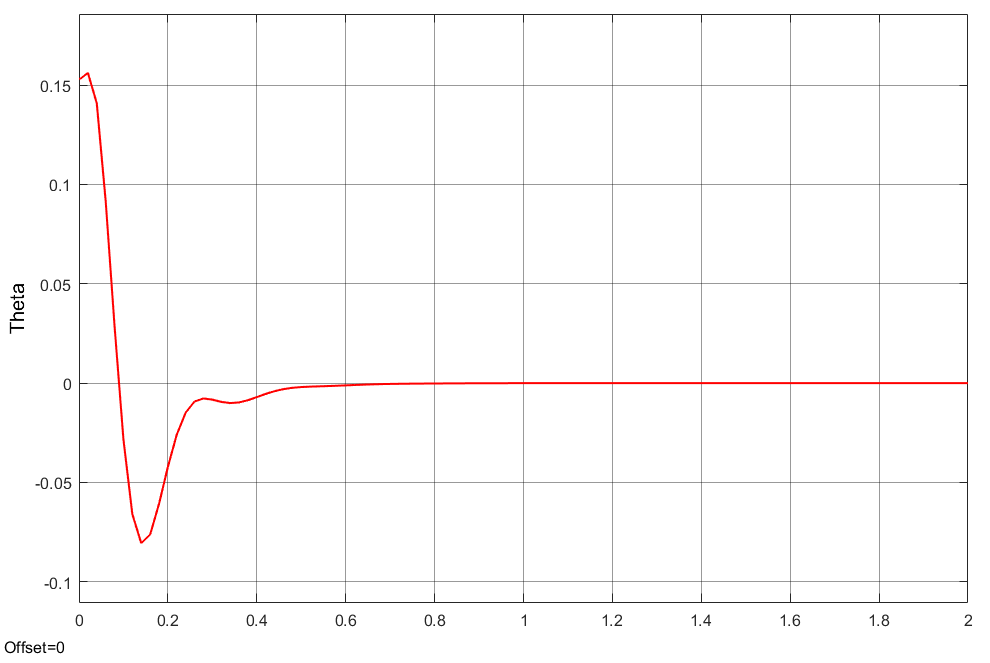
\includegraphics[scale=0.5]{Task_14_01.png}
    \caption{The step response of the system with $\tau=0.01$}
    \label{fig:16}
\end{figure}

\begin{figure}[H]
    \centering
    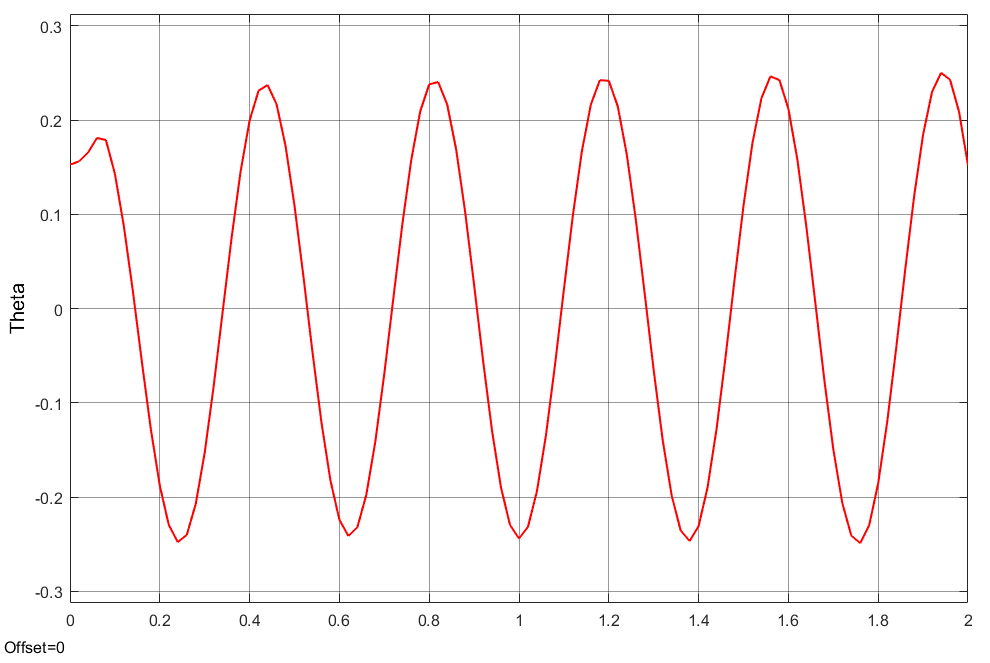
\includegraphics[scale=0.5]{Task_14_04.png}
    \caption{The step response of the system with $\tau=0.04$}
    \label{fig:17}
\end{figure}

\begin{figure}[H]
    \centering
    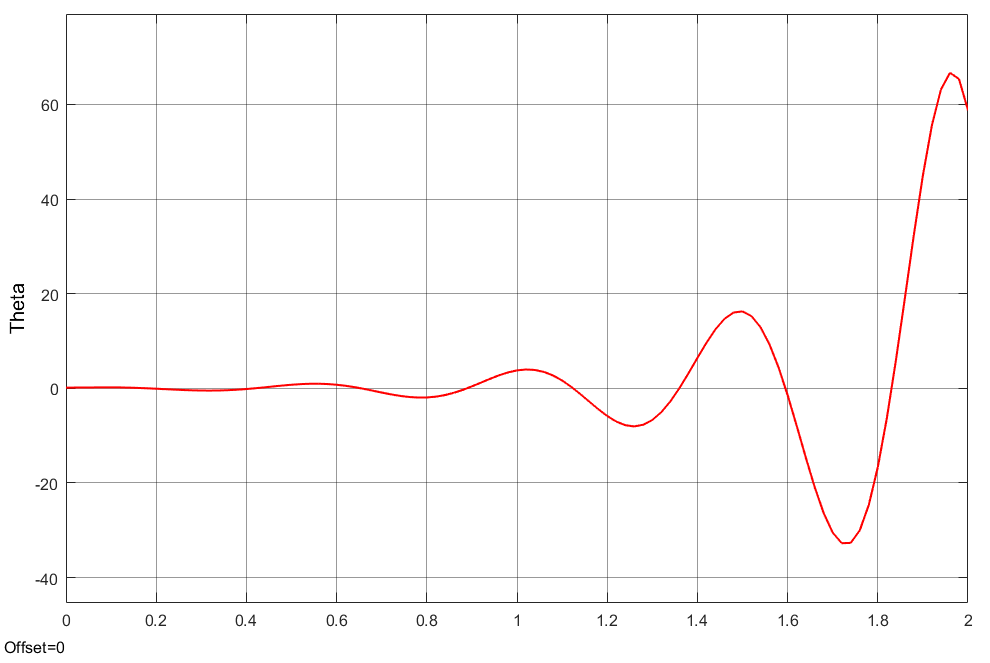
\includegraphics[scale=0.5]{Task_14_06.png}
    \caption{The step response of the system with $\tau=0.06$}
    \label{fig:18}
\end{figure}


\section*{Task 15}
The formal definition of $\tau_i$ as following.
\begin{equation}
    \tau_i =  (S_i,S_{0_i} ,Act_i, \rightarrow_i, AP_i, L_i)
\end{equation}
From the graph the following relations can be derived:

For the first system $\tau_1$: 
$S_1 = \{s_0, s_1, s_2\}$, $S_{0_1} = \{s_{0_0}, s_{0_1}, s_{0_2}\}$, $Act_1 = \{a, b, c\}$, 
$\rightarrow_1 = \{(s_0, a, s_1), (s_1, c, s_0), (s_2, b, s_0), (s_1, a, s_2)\}$ 

For the second system $\tau_2$: 
$S_2 = \{t_0, t_1, t_2\}$, $S_{0_2} = \{t_{0_0}, t_{0_1}, t_{0_2}\}$, $Act_2 = \{a, b, c\}$, 
$\rightarrow_1 = \{(t_0, a, t_1), (t_1, c, t_2), (t_2, c, t_0), (t_0, b, t_2)\}$

\section*{Task 16}
The product interleaving transition system $\tau_{int}$ shall have the following parameters: 
$\tau_{int} = (S_{int}, S_{0_{int}}, Act_{int}, \rightarrow_{int}, AP_{int}, L_{int} )$. Here:
\begin{equation}
\begin{aligned}
    S_{int} & = \{(s_0, t_0), (s_1, t_0), (s_2, t_0), (s_0, t_1), (s_1, t_1), (s_2, t_1), (s_0, t_2), (s_1, t_2), (s_2, t_2)\} \\
    S_{int}^0 & = \{(S_1^0, S_2^0)\} \\
    Act_{int} & = \{a, b, c\} \\
    \rightarrow_{int} & = \{((s_0, t_i), a, (s_1, t_i)), ((s_1, t_i), c, (s_0, t_i)), ((s_2, t_i), b, (s_0, t_i)), ((s_1, t_i), a, (s_2, t_i)), \\ 
    & ((s_i, t_0), a, (s_i, t_1)), ((s_i, t_1), c, (s_i, t_2)), ((s_i, t_2), c, (s_i, t_0)), ((s_i, t_0), b, (s_i, t_2))\} \\ & \forall i = 1,2,3
\end{aligned}
\end{equation}

\section*{Task 17}
The product handsharking transition system $\tau_{hand}$ shall have the following parameters: 
$\tau_{hand} = (S_{hand}, S_{0_{hand}}, Act_{hand}, \rightarrow_{hand}, AP_{hand}, L_{hand} )$. Here for $H = \{c\}$:
\begin{equation}
\begin{aligned}
    S_{int} & = \{(s_0, t_0), (s_1, t_0), (s_2, t_0), (s_0, t_1), (s_1, t_1), (s_2, t_1), (s_0, t_2), (s_1, t_2), (s_2, t_2)\} \\
    S_{int}^0 & = \{(S_1^0, S_2^0)\} \\
    Act_{int} & = \{a, b, c\} \\
    \rightarrow_{int} & = \{((s_0, t_i), a, (s_1, t_i)), ((s_2, t_i), b, (s_0, t_i)), ((s_1, t_i), a, (s_2, t_i)), ((s_i, t_0), a, (s_i, t_1)), \\
    & ((s_i, t_0), b, (s_i, t_2)), ((s_1, t_1), c, (s_0, t_2)), ((s_1, t_2), c, (s_0, t_0))\} \forall i = 1,2,3
\end{aligned}
\end{equation}


%%%%%%%%%%%%%%%%%%%%%%%%%%%%%%%%%%%%%%%%%%%%%%%%%%%%%%%%%%%%%%%%%%%%%%%%%%%%%%%%%%%
% The bibliography
%%%%%%%%%%%%%%%%%%%%%%%%%%%%%%%%%%%%%%%%%%%%%%%%%%%%%%%%%%%%%%%%%%%%%%%%%%%%%%%%%%%
%\bibliography{Bibliography_template} %Read the bibliography from a separate file

\begin{thebibliography}{99}
\bibitem[Khalil(2002)]{Khalil:2002:Nonlinear-systems:vh}
Hassan~K Khalil.
\newblock \emph{Nonlinear systems}.
\newblock Prentice Hall, Upper Saddle river, 3. edition, 2002.
\newblock ISBN 0-13-067389-7.

\bibitem[Oetiker et~al.(2008)Oetiker, Partl, Hyna, and
  Schlegl]{Oetiker:2008:TheNotSoShortIntroductiontoLaTeXe}
Tobias Oetiker, Hubert Partl, Irene Hyna, and Elisabeth Schlegl.
\newblock \emph{The Not So Short Introduction to \LaTeXe}.
\newblock Oetiker, OETIKER+PARTNER AG, Aarweg 15, 4600 Olten, Switzerland,
  2008.
\newblock http://www.ctan.org/info/lshort/.

\bibitem[Sastry(1999)]{Sastry:1999:Nonlinear-systems:-analysis-stability-and-c%
ontrol:xr}
Shankar Sastry.
\newblock \emph{Nonlinear systems: analysis, stability, and control},
  volume~10.
\newblock Springer, New York, N.Y., 1999.
\newblock ISBN 0-387-98513-1.
\end{thebibliography}


\end{document}      % End of the document
